%!TEX root = ../thesis.tex

\section{Blue face subdivision}

\paragraph{Assumptions}
At this point we have a vertically one-sided graph without large (4 or more edges) topfans. Due to flipping topfans we don't know where exactly we have split and merge vertices. Due to topfanflips not overlapping we know that the splits are small \fxwarning{TODO is this true? I hope it is}

\paragraph{Goal}
We want to recolor edges in each blue face such that in the subdivision of that face every blue face is 3-sided.


\paragraph{How}
We flip edges in each face, taking into account loads on the bottom fence. Such that

\begin{enumerate}
  \item We never load the edge next to a split/merge
  \item We never load two adjecent edges
\end{enumerate}

It's important to note that we put trough edge loads on splits and merges

Because we do this we can also say the following

\begin{lemma}
  \label{lm:}
  On the bottom boundary path of every face we never find two subsequent loaded edges. Even when we put trough loads on splits and merges.
\end{lemma}
\begin{proof}
  A single face would never load two subsequent edges. Hence the only way to get two subsequent loaded edges is using different faces and thus splits and merges.

  However due to the built-in safety of never flipping next to a split/merge we never get subsequent    loaded edges.
  \fxnote{Might add a figure}
\end{proof}

\begin{lemma}
  \label{lm:}
  We can subdivide any blue face without large topfans into 7-sided chunks while obeying the load rules above.
  \fxnote{We can make this Lemma WAY tighter if all topfans are of size exactly 2}
\end{lemma}

\begin{proof}
  A worst case example is given in Figure \ref{fig:subdiv:worstCase}.

  \begin{figure}[h]
    \centering
    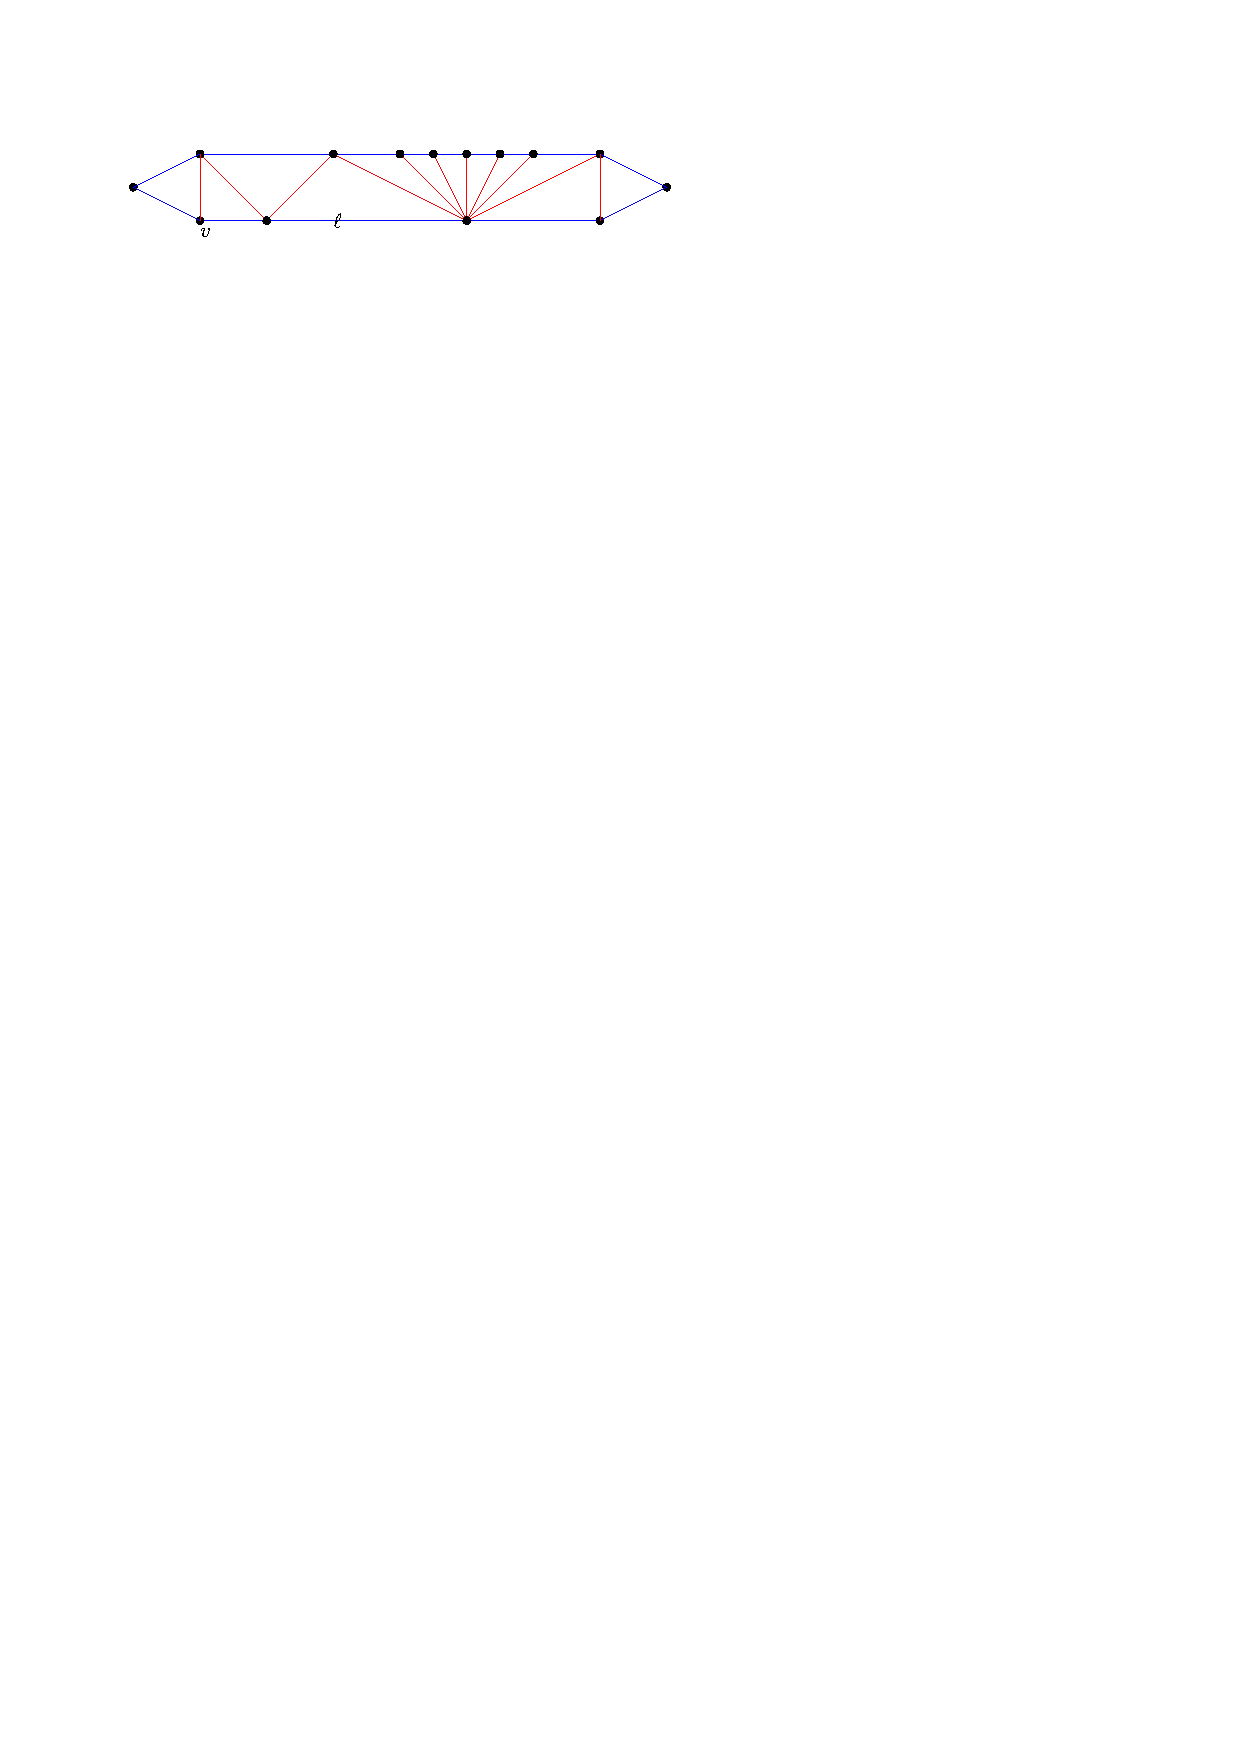
\includegraphics[scale=1]{blueFaceSubdivision/img/worstCase}
    \caption{A worst case blue face. We don't flip any edge in this face.}
    \label{fig:subdiv:worstCase}
  \end{figure}

  Note that we can flip above each edge in the bottom boundary path.

  We will look at the vertex on the bottom fence that's adjacent to the freshly flipped edge,  or if we haven't flipped an edge yet the vertex next to the split (and we will call it $v$). The following are then the rules for flipping above the edges following $v$.
  \begin{enumerate}
    \item We don't flip above the first three edges.
    \item We flip above the fourth edge if it's unloaded.
    \item We flip above the fifth edge if it's not next to (or next to next to) the merge
    \item Otherwise the sixth or seventh edge is followed by the merge
  \end{enumerate}

The first three edges give us the required separation of loaded edges along the top boundary path. The other items make sure we obey the other rules in a straightforward manner. If we arrive at the fifth edge the fourth edge was loaded and thus the fifth one isn't.

See Figure \ref{fig:subdiv:sampleExecution} for an example of an execution of this algorithm.

\begin{figure}[h]
  \centering
  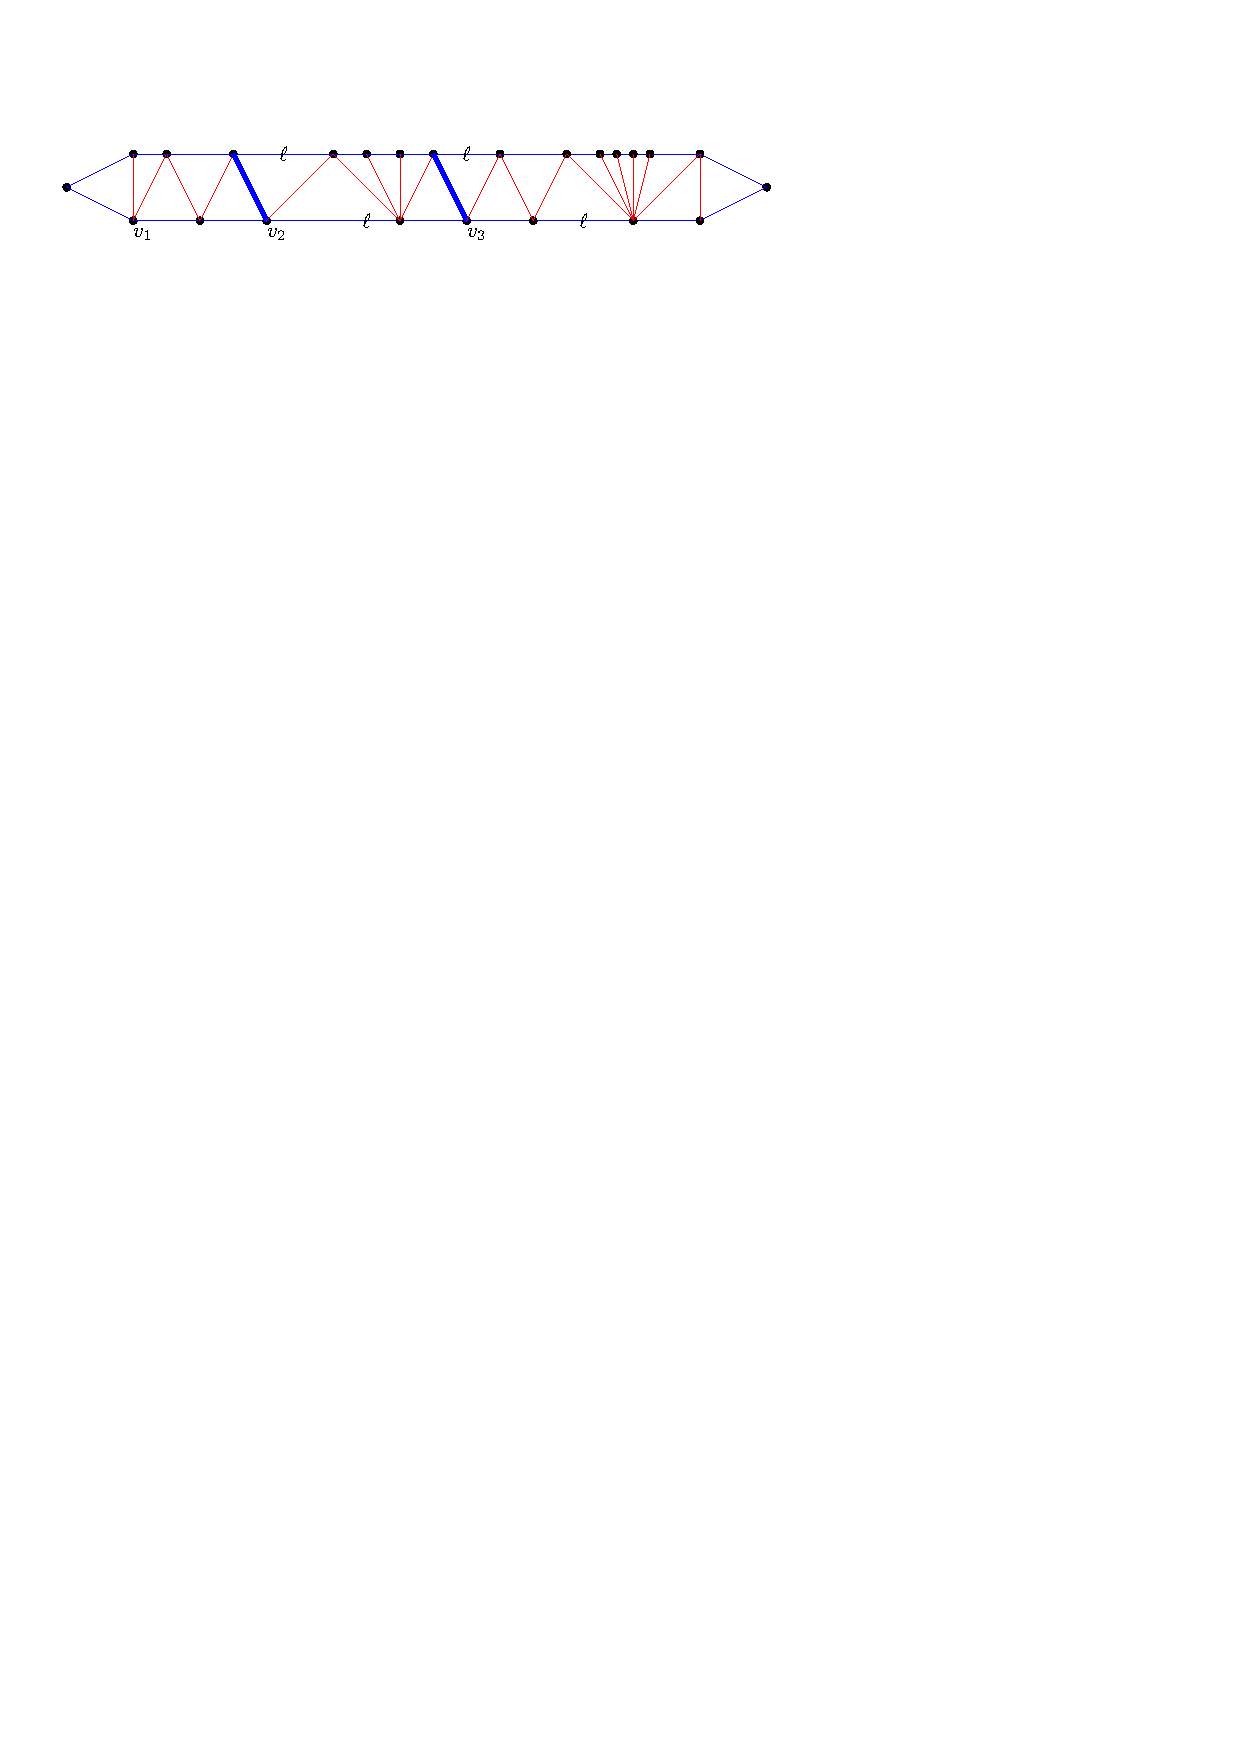
\includegraphics[scale=1]{blueFaceSubdivision/img/sampleExecution}
  \caption{Sample execution of the algorithm}
  \label{fig:subdiv:sampleExecution}
\end{figure}

\end{proof}


\begin{lemma}
  \label{lm:}
  We have a 7-sided REL
\end{lemma}

\begin{proof}
  By construction a blue faces are 7-sided. We haven't chained $Z's$ so all red face contain at most one blue $Z$. Because fanflips are not layered the largest split is of size two. So red faces are 3-sided.
  \fxerror{This doesn't account for south-adjecent vertices. Maybe make the goal dependen on size of southadjecent vertices.}
\end{proof}
